\subsection{Herstellung der Compact Disc}
\label{subsec:cdherstellung}

Die Herstellung einer CD beginnt mit der Anfertigung einer Glasmatrize. Diese
besteht aus einer Glasplatte und einer Fotolackschicht, welche die Pitstruktur
enthält. Aus dieser wird daraufhin eine Metallmatrize gefertigt, welche für das
Spritzgussverfahren verwendet wird. Dabei wird die Matrize in das flüssige
Polycarbonat gepresst. Dadurch überträgt sich die Pitstruktur, wie in
\autoref{fig:cdherstellung}, auf die Polycarbonatscheibe. Auf diese wird
anschließend das Aluminium aufgedampft, um die Reflexionsschicht zu erhalten,
und mithilfe einer Schutzschicht versiegelt. \cite{cdp}

\begin{figure}[h]
  \begin{center}
      \begin{minipage}[t]{\textwidth}
        \begin{center}
            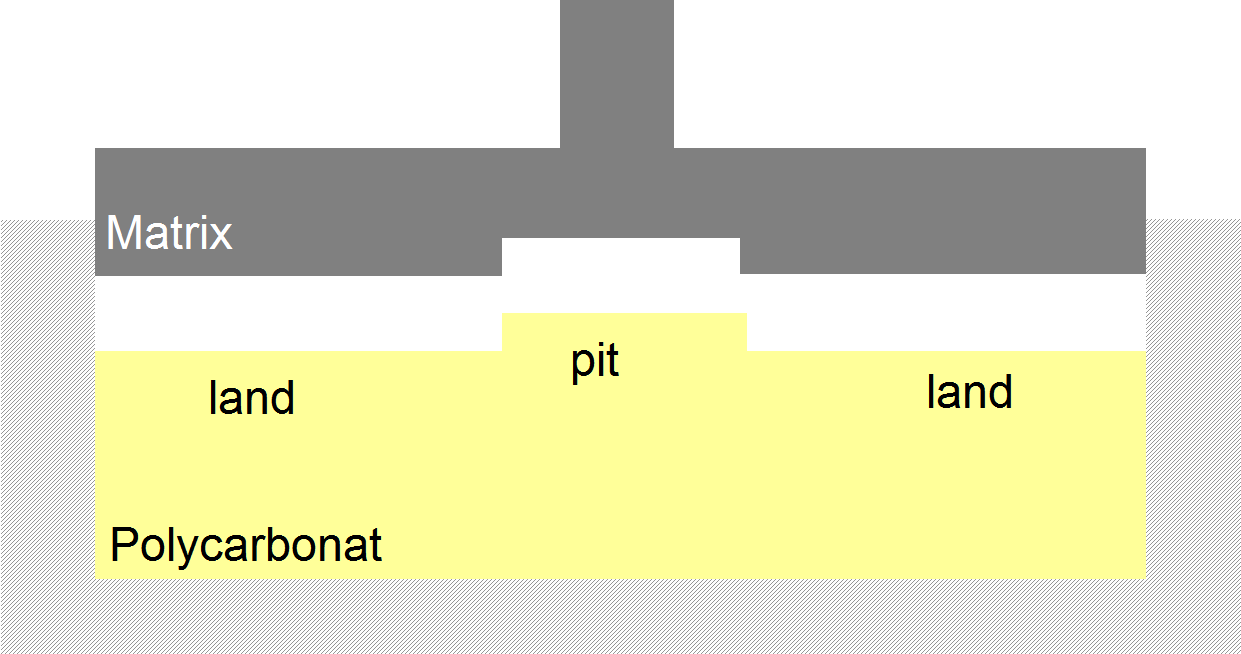
\includegraphics[height=0.1\textheight]{Bilder/Optische_Datentraeger_Die_Compact_Disc/Herstellung/cdherstellung.png}
            \caption[Spritzgussverfahren \newline \url{http://daten.didaktikchemie.uni-bayreuth.de/umat/cd_dvd/spritzguss.gif} (zuletzt aufgerufen am 07.08.2015)]{Spritzgussverfahren}
            \label{fig:cdherstellung}
        \end{center}
      \end{minipage}
  \end{center}
\end{figure}
